\section{Auswertung}
\label{sec:Auswertung}

\subsection{Charakteristik des Zählrohrs}
\label{ssec:charakteristik_auswertung}

\begin{table}
    \centering
    \caption{Messergebnisse der Charakteristik des Zählrohrs}
    \begin{tabular}{S[table-format=3.0] S[table-format=5.0]}
        \toprule
        \tableSI{U}{\volt} & \tableSI{N}{\frac{Imp}{60\second}} \\
        \midrule
        320 & 9672 \\
        330 & 9689 \\
        340 & 9580 \\
        350 & 9837 \\
        360 & 9886 \\
        370 & 10041 \\
        380 & 9996 \\
        390 & 9943 \\
        400 & 9995 \\
        410 & 9980 \\
        420 & 9986 \\
        430 & 9960 \\
        440 & 10219 \\
        \bottomrule
    \end{tabular}
    \begin{tabular}{S[table-format=3.0] S[table-format=5.0]}
        \toprule
        \tableSI{U}{\volt} & \tableSI{N}{\frac{Imp}{60\second}} \\
        \midrule
        450 & 10264 \\
        460 & 10174 \\
        470 & 10035 \\
        480 & 10350 \\
        490 & 10290 \\
        500 & 10151 \\
        510 & 10110 \\
        520 & 10255 \\
        530 & 10151 \\
        540 & 10351 \\
        550 & 10184 \\
        560 & 10137 \\
        570 & 10186 \\
        \bottomrule
    \end{tabular}
    \begin{tabular}{S[table-format=3.0] S[table-format=5.0]}
        \toprule
        \tableSI{U}{\volt} & \tableSI{N}{\frac{Imp}{60\second}} \\
        \midrule
        580 & 10171 \\
        590 & 10171 \\
        600 & 10253 \\
        610 & 10368 \\
        620 & 10365 \\
        630 & 10224 \\
        640 & 10338 \\
        650 & 10493 \\
        660 & 10467 \\
        670 & 10640 \\
        680 & 10939 \\
        690 & 11159 \\
        700 & 11547 \\
        \bottomrule
    \end{tabular}
    \label{tab:charakteristik}
\end{table}

Die Charakteristik des benutzten Zählrohrs ist in \autoref{fig:plot_charakteristik} dargestellt.
Um den Plateauanstieg zu bestimmen wird eine Ausgleichsgerade durch das Plateau (also von $U=$ \SIrange{370}{640}{\volt}) gelegt.
Dazu wird 
\begin{equation*}
    N(U) = aU + b
\end{equation*}
und die Funktion curve\_fit der Python Bibliothek SciPy verwendet.\cite{scipy}
Damit ergeben sich die Parameter
\begin{align*}
    a &= \SI{0.019+-0.004}{\per\volt} \\
    b &= \SI{160+-2}{} \, .
\end{align*}
Nun kann der Plateauanstieg zu
\begin{align*}
    \Delta N &= N(U=\SI{640}{\volt}) - N(U=\SI{370}{\volt}) \\
             &= \SI{5.2+-1.0}{\frac{Imp}{\second}}
\end{align*}
bzw.
\begin{align*}
    \Delta N &= \left( \frac{N(U=\SI{640}{\volt})}{N(U=\SI{370}{\volt})} - 1 \right) \cdot \frac{\SI{100}{\volt}}{(640-370)\:\si{\volt}} \cdot 100 \\
             &= \SI{1.15+-0.21}{\percent\per100\volt}
\end{align*}
bestimmt werden.

\begin{figure}
    \centering
    \includegraphics[width=\textwidth]{build/plot_charakteristik.pdf}
    \caption{Plot der Messergebnisse aus \autoref{tab:charakteristik} mit passendem Fehler $\Delta N = \sqrt{N}$ und Ausgleichsgerade}
    \label{fig:plot_charakteristik}
\end{figure}


\subsection{Totzeit des Zählrohrs}
\label{ssec:totzeit_auswertung}

Wie in Abschnitt \ref{ssec:totzeit_durchführung} beschrieben wurde zunächst die Zwei-Quellen-Methode zur untersuchung der Totzeit verwendet.
Hier ergab die Messung
\begin{align*}
    N_1 &= \:\:\SI{96041}{\frac{Imp}{120\second}} \\
    N_{1+2} &= \SI{158479}{\frac{Imp}{120\second}} \\
    N_2 &= \:\:\SI{76518}{\frac{Imp}{120\second}} \, .
\end{align*}

Nun kann wegen der Totzeitkorrektur
\begin{equation}
    N_\text{geschätzt} = \frac{N_\text{gemessen}}{1-T \cdot N_\text{gemessen}}
\end{equation}
und
\begin{equation}
    N_\text{1+2,geschätzt} = N_\text{1,geschätzt} + N_\text{2,geschätzt}
\end{equation}
die Totzeit über
\begin{equation}
    T = \frac{N_1 + N_2 - N_\text{1+2}}{2 \cdot N_1 \cdot N_2}
\end{equation}
abgeschätzt werden.
Somit ergibt sich aus der Zwei-Quellen-Methode eine Totzeit 
\begin{equation*}
    T = \SI{115+-4}{\micro\second} \, .
\end{equation*}

Die zweite in Abschnitt \ref{ssec:totzeit_durchführung} beschriebene Methode führt zur \autoref{fig:oszilloskop}. 
\begin{figure}
    \centering
    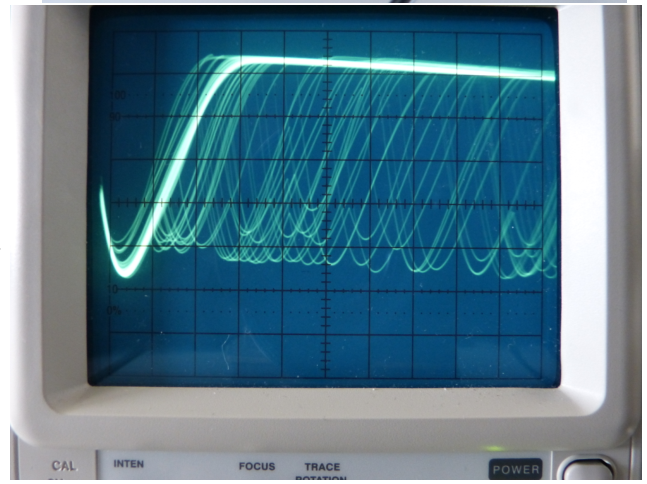
\includegraphics[width=0.7\textwidth]{images/oszilloskop.png}
    \caption{Oszillogram zur Schätzung der Totzeit wobei ein Kästchen horizontal $\SI{100}{\micro\second}$ entspricht}
    \label{fig:oszilloskop}
\end{figure}
Hier kann die Zeitdifferenz des ersten zum zweiten Puls sehr grob abgelesen werden.
So ergibt sich eine Totzeit von
\begin{equation*}
    T = \SI{100+-100}{\micro\second} \, .
\end{equation*}


\subsection{Bestimmung der pro Teilchen vom Zählrohr freigesetzten Ladungen}
\label{ssec:ladungen_auswertung}

\begin{table}
    \centering
    \caption{Messergebnisse des Vergleichs der Stromstärke zur Intensität}
    \begin{tabular}{S[table-format=3.1(1)] S[table-format=1.2(2)] S[table-format=1.1(1)]}
        \toprule
        \tableSI{N}{\frac{Imp}{\second}} & \tableSI{I}{\micro\ampere} & \tableSI{Z}{10^{10}} \\
        \midrule
        163.9+-1.7 & 0.3+-0.05 & 1.1+-0.2 \\
        166.6+-1.7 & 0.4+-0.05 & 1.5+-0.2 \\
        171.1+-1.7 & 0.7+-0.05 & 2.6+-0.2 \\
        169.2+-1.7 & 0.8+-0.05 & 3.0+-0.2 \\
        169.7+-1.7 & 1.0+-0.05 & 3.7+-0.2 \\
        170.9+-1.7 & 1.3+-0.05 & 4.7+-0.2 \\
        174.9+-1.7 & 1.4+-0.05 & 5.0+-0.2 \\
        192.4+-1.8 & 1.8+-0.05 & 5.8+-0.2 \\
        \bottomrule
    \end{tabular}
    \label{tab:strom}
\end{table}

Beim Aufnehmen der Charakteristik wurde zusätzlich noch im Abstand von $\SI{50}{\volt}$ die Ionisierungsstromstärke $I$ gemessen.
Aus den gemessenen Werten kann die Zahl der freigesetzten Ladungen pro detektiertem Teilchen über
\begin{equation}
    Z = \frac{I}{e \cdot N}
\end{equation}
berechnet werden, wobei $e=\SI{1.602e-19}{\coulomb}$ die Elementarladung ist.
Die so berechneten $Z$ sind in \autoref{tab:strom} aufgelistet und in \autoref{fig:plot_strom} dargestellt.

\begin{figure}
    \centering
    \includegraphics[width=\textwidth]{build/plot_strom.pdf}
    \caption{Plot der Ergebniss aus \autoref{tab:strom}}
    \label{fig:plot_strom}
\end{figure}